\section{Introduzione}

In questo progetto ho implementato la soluzione per la determinazione delle K
migliori soluzioni del problema monodimensionale di knapsack proposta in
\cite{YANASSE2000}.

\begin{align*}
  \{z_1,z_2,\cdots,z_K\} \in & \{\sum\limits_{i=1}^n c_ix_i\}\\
  z_j = \max\limits_x & \{\{\sum\limits_{i=1}^n c_ix_i\}\backslash\{z_h\}_{h=1}^{j-1}\}& j = [1,K]\\
%
  &\sum\limits_{i=1}^n a_ix_i \le b\\
  &x_i\ge0, intero
\end{align*}

Dove $K$ è il numero di soluzioni richieste, $z_j$ è la $j-esima$ soluzione
ottima, $\bar{x}$ è il vettore delle soluzioni, $\bar{c}$ è il vettore dei
costi, $\bar{a}$ è il vettore dei pesi e $b$ è il peso massimo.

Nell'articolo, gli autori propongono uno schema enumerativo di complessità
temporale $O(Knb)$ e spaziale $O(nb)$.

\section{Algoritmo}

Considero $n$ elementi con pesi $\bar{w}=\{w_1, w_2, \cdots, w_n\}$ e valori
$\bar{a}=\{a_1, a_2, \cdots,a_n\}$, tali che $w_1 \le w_2 \le \cdots \le w_n$.
L'algoritmo si suddivide in due parti: una ricerca \emph{forward} ed una
\emph{backward}. Poich\'e l'algoritmo è descritto in dettaglio in
\cite{YANASSE2000}, mi limito a riportare un breve riassunto incentrato sulla
sua implementazione piuttosto che sull'aspetto teorico.

\subsection{Ricerca forward}

La ricerca forward porta a determinare al più $n$ migliori
valori per ogni $w \in [w_1;b]$. Per ogni valore non si memorizza il vettore
delle soluzioni ma solo l'indice dell'elemento più pesante presente in
soluzione.

La ricerca si effettua utilizzando una matrice $b\times{}n$, in cui nella riga
$i-esima$ risiedono al più $n$ migliori soluzioni con peso totale $i$.
L'indice di colonna $j$ è uguale all'indice dell'elemento più pesante presente
in soluzione.

Il risultato della ricerca \emph{forward} sono $K$ valori, di cui il migliore
di essi corrisponde al valore della migliore soluzione del problema.

\subsection{Ricerca backward}

La ricerca backward utilizza la matrice della ricerca forward per ricostruire
il vettore delle soluzioni per ognuno dei $K$ valori individuati. Per ogni
valore $v_{i,j}$ si conoscono gli indici $i,j$ che sono rispettivamente il peso
della soluzione e l'elemento più pesante in soluzione. Stabilito $i' = i -
w_j$, la matrice contiene un elemento di valore $v_{i',j'} = v_{i,j} - v_l$
nella riga di indice $i'$, colonna $j'$. Noto il vettore soluzioni $\bar{X}$
che porta in ${i',j'}$, si può ottenere la soluzione in ${i,j}$, aggiungengo
$1$ ad $X_j$.

La ricerca di una singola soluzione termina quando, supponendo $i,j$ gli indici
correnti, $i - w_j = 0$.

Tuttavia le soluzioni cos\`i ottenute non sono necessariamente le $K$ migliori
soluzioni, poich\'e la matrice generata dalla ricerca forward contiene i
migliori valori per ogni peso, ma potrebbero esistere soluzioni di peso $j_a$,
non presenti nella matrice, con valore maggiore di soluzioni presenti in
qualsiasi $j_b \neq j_a$.

Per risolvere questo problema, durante la ricerca backward si cercano soluzioni
alternative, esplorando gli altri valori presenti nella riga corrente, fissata
la soluzione parziale corrente.

\section{Implementazione}

L'algoritmo è stato implmementato in \code{C}, realizzando una libreria che
offre una interfaccia per dichiarare e risolvere il problema.

Il progetto è gestito da \code{CMake} e la documentazione da \code{doxygen},
dunque i commenti sopra le signature delle funzioni ne descrivono parametri e
comportamento. Istruzioni su come usare \code{cmake} per creare un progetto
sono nel \code{README.md} nella root del progetto. Il progetto è su \code{github}:
\url{https://github.com/dbellavista/MMSD1213_knapsackKbest}.

Nella cartella \code{src/demo} è presente una piccola demo che utilizza la
libreria.

\subsection{Problema di soluzioni identiche}

La ricerca delle soluzioni alternative trova soluzioni che sono ottenute
esplorando strade diverse, ma che portano allo stesso risultato, ovvero lo
stesso vettore delle soluzioni. Questo comportamento lo si nota anche
nell'esempio riportato dall'articolo, ma non lo si menziona. Nella sottosezione
\emph{Recovering the K-best solutions}, paragrafo 7 (in fondo alla pagina), si
descrive il processo di recovering di soluzioni alternative per il valore $19$.

Nel processo di \emph{recovering} (ricerca backward), dalla riga $15$ si passa
alla riga $9$, con una soluzione parziale di valore $7$. Esplorando le
alternative, si trova un valore $11+7 = 18$, che è inserito nelle soluzioni.
Riprendendo la ricerca backward per $19$, si sottrae $3$, arrivando alla riga
$6$ con una soluzione parziale di valore $11$. La nuova soluzione ha un vettore
delle soluzioni pari a $[3,0,0,1,0]$.

L'articolo non lo menziona, ma esplorando le soluzioni alternative, si arriva
ad una soluzione $7 + 11=18$ che andrebbe inserita nella lista di soluzioni, ma
il suo vettore delle soluzioni ($[3,0,0,1,0]$) è identico alla soluzione
alternativa trovata precedentemente.

Per evitare questi problemi, ho implementato un controllo efficiente per
verificare l'univocità delle soluzioni utilizzando principalmente una bitmap in
cui il bit $jesimo$ vale $0$ se $x_j=0$ e vale $1$ se $x_j > 0$.

\section{Risultati}

Non sono riuscito ad ottenere le stesse performance riportate nell'articolo.
Generando problemi random utilizzando il generatore in
\url{http://www.diku.dk/~pisinger/codes.html}, ho ottenuto istanze risolvibili
in tempi irrisori perch\'e le soluzioni ottime erano composte in gran parte
dall'elemento più leggero, mentre altre istanze erano estremamente difficili e
i tempi largamente maggiori da quelli riportati nell'articolo.

Ho effettuato un test con $20$ problemi random con $n = 500$, $b = 10.000$, $w_i
\in [1,5.000]$, per valori di $K$ pari a $100, 200, 300, 400, \dots, 1.200$.

In figura\ref{fig:var_k}, è riportato il grafico dell'andamento del tempo
computazionale.

\begin{figure}[!h]
  \centering
  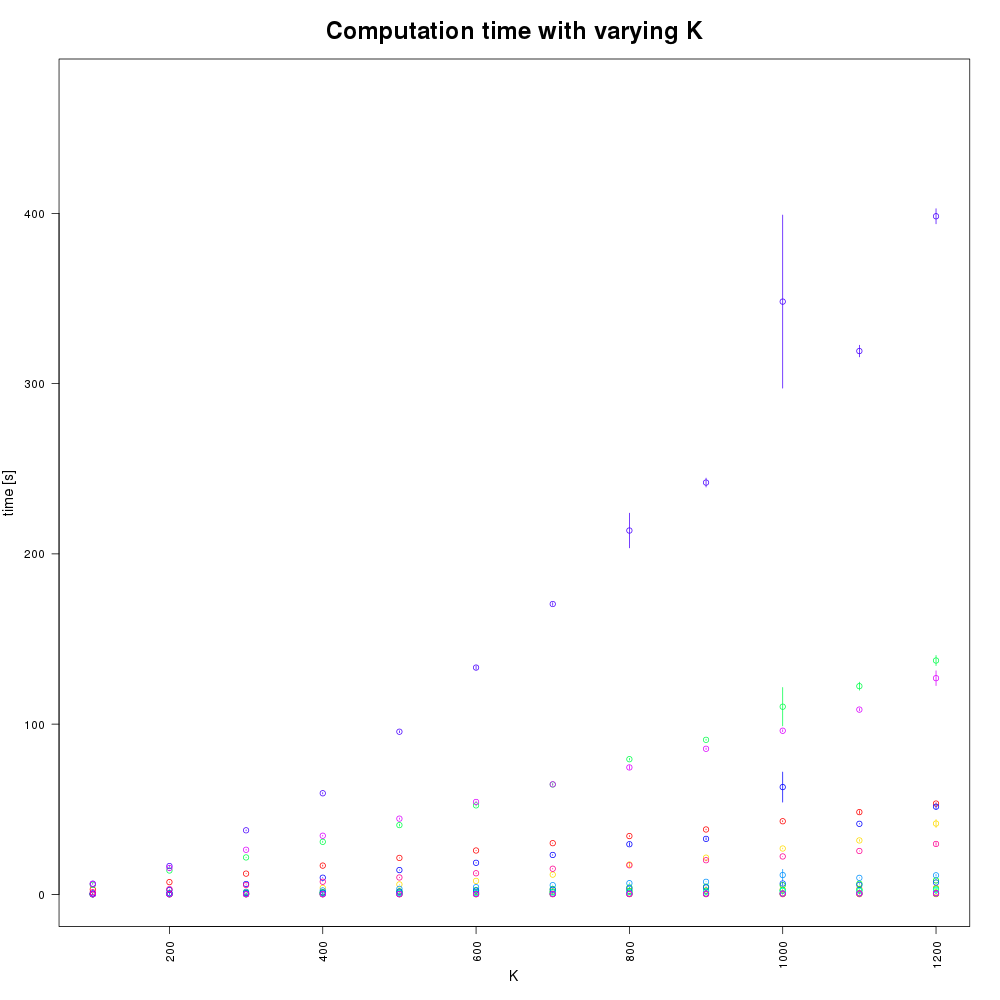
\includegraphics[width=12cm]{./imgs/variation_K.png}
  \caption{Tempo computazionale al variare di $K$, con $n = 500$, $b = 10.000$
  su $20$ problemi. Ad ogni colore corrisponde un problema}
  \label{fig:var_k}
\end{figure}
